
%%%%%%%%%%%%%%%%%%%%%%%%%%%%%%%%%%%%%
% Document properties and packages
%%%%%%%%%%%%%%%%%%%%%%%%%%%%%%%%%%%%%
\documentclass[a4paper,12pt,final]{memoir}

% misc
\renewcommand{\familydefault}{bch}	% font
\pagestyle{empty}					% no pagenumbering
\setlength{\parindent}{0pt}			% no paragraph indentation


% required packages (add your own)
\usepackage{flowfram}										% column layout
\usepackage[top=1cm,left=1cm,right=1cm,bottom=1cm]{geometry}% margins
\usepackage{graphicx}										% figures
\usepackage{url}											% URLs
\usepackage[usenames,dvipsnames]{xcolor}					% color
\usepackage{multicol}										% columns env.
	\setlength{\multicolsep}{0pt}
\usepackage{paralist}										% compact lists
\usepackage{tikz}
%%%%%%%%%%%%%%%%%%%%%%%%%%%%%%%%%%%%%
% Create column layout
%%%%%%%%%%%%%%%%%%%%%%%%%%%%%%%%%%%%%
% define length commands
\setlength{\vcolumnsep}{\baselineskip}
\setlength{\columnsep}{\vcolumnsep}

% frame setup (flowfram package)
% left frame
\newflowframe{0.2\textwidth}{\textheight}{0pt}{0pt}[left]
	\newlength{\LeftMainSep}
	\setlength{\LeftMainSep}{0.2\textwidth}
	\addtolength{\LeftMainSep}{1\columnsep}
 
% small static frame for the vertical line
\newstaticframe{1.5pt}{\textheight}{\LeftMainSep}{0pt}
 
% content of the static frame
\begin{staticcontents}{1}
\hfill
\tikz{%
	\draw[loosely dotted,color=RoyalBlue,line width=1.5pt,yshift=0]
	(0,0) -- (0,\textheight);}%
\hfill\mbox{}
\end{staticcontents}
 
% right frame
\addtolength{\LeftMainSep}{1.5pt}
\addtolength{\LeftMainSep}{1\columnsep}
\newflowframe{0.7\textwidth}{\textheight}{\LeftMainSep}{0pt}[main01]
%%%%%%%%%%%%%%%%%%%%%%%%%%%%%%%%%%%%%
% define macros (for convience)
%%%%%%%%%%%%%%%%%%%%%%%%%%%%%%%%%%%%%
\newcommand{\Sep}{\vspace{1.5em}}
\newcommand{\SmallSep}{\vspace{0.5em}}

\newenvironment{AboutMe}
	{\ignorespaces\textbf{\color{RoyalBlue} About me}}
	{\Sep\ignorespacesafterend}
	
\newcommand{\CVSection}[1]
	{\Large\textbf{#1}\par
	\SmallSep\normalsize\normalfont}

\newcommand{\CVItem}[1]
	{\textbf{\color{RoyalBlue} #1}}
%my macro
\newcommand{\test}[1]
	{\underline{\textbf{\color{RoyalBlue} #1:}}\vspace{4pt}}	
%%%%%%%%%%%%%%%%%%%%%%%%%%%%%%%%%%%%%
% Begin document
%%%%%%%%%%%%%%%%%%%%%%%%%%%%%%%%%%%%%
\begin{document}
% Left frame
%%%%%%%%%%%%%%%%%%%%
\begin{figure}
	\hfill
	\center
	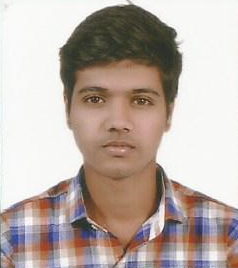
\includegraphics[width=0.6\columnwidth]{kashif}
	\vspace{-7cm}	
	

\end{figure}

\begin{center}\small
	R-20/5,Jaitpur \\
	\hspace{-5pt}Badarpur,\\New Delhi-110044	\\\vspace{1pt}
	\url{kashifnoori14@gmail.com}\\\vspace{1pt}
	+91-8527144896	
	%\url{www.howtotex.com} \\
	 
\end{center}\normalsize
\framebreak
% Right frame
%%%%%%%%%%%%%%%%%%%%
\Huge\bfseries {\color{RoyalBlue} Kashif Khurshid Noori} \\
%\Large\bfseries  Graphics designer \\

\normalsize\normalfont
\CVSection{Career Objective}
I wish to pursue a career in the field of Autonomous Mobile Robots that I can help to resolve common issues being faced day in day out. For this I want to be a part of a progressive organization that gives me a scope to enhance and upgrade my knowledge and utilize my skills towards the sustainable growth of the society.\\

% Experience
\CVSection{Academic Details}

\indent \begin{tabular}{ l l l l}
\hline
\textbf{\color{RoyalBlue}Examination} & \textbf{\color{RoyalBlue}Institute} & \textbf{\color{RoyalBlue}Year} & \textbf{\color{RoyalBlue}CPI/\%} \\
\hline
UnderGraduate Specialization:\,\, & \textit{E \& C Engineering} \\
Graduation & FET JMI & 2020 & 7.68 \\
\hline
%UnderGraduate Specialization: & \textit{Computer Engineering} \\
Senior Secondary/+2 & S.A.H Sr. Sec. School & 2016 & 84.2\\
\hline
\end{tabular}
\Sep
%interest

\CVSection{Field of Interest}

\begin{compactitem}[\color{RoyalBlue}$\circ$]
\item\noindent I have a pristine interest in Autonomous Robots. I wish to altruistically contribute towards development of a robust robot based on ROS and Embedded systems.
\end{compactitem}
\SmallSep

% Skills
\CVSection{Technical Skills}
\CVItem{Languages:}
\\
\begin{tabular}{l l}
C/Embedded C, C++ & Intermediate\\
Python & Beginners
\end{tabular} 
\\
\CVItem{Tools/Platforms:}
\\
\begin{tabular}{l l}
Arduino, Atmel Studio & Intermediate\\
Robot Operating System & Beginners\\

\end{tabular}
\Sep

%soft skills
\CVSection{Soft Skills}
\begin{tabular}{@{\color{RoyalBlue}$\circ$\hspace{4pt}}l @{\hskip 15pt\color{RoyalBlue}$\circ$\hspace{4pt}} l@{\hskip 15pt\color{RoyalBlue}$\circ$\hspace{4pt}}l}
Positive Attitude & Accept Constructive Criticism & Flexibility\\
\vspace{10pt}
Working as a team & Leadership & Critical thinking
\end{tabular}
\Sep\vspace{9pt}
%projects
\CVSection{Projects}\vspace{-25pt} 
\begin{compactitem}[\color{RoyalBlue}]
\item\test{1. Transporter Bot}
\subitem -It is two wheeled diffrential drive robot based on FireBirdV and \subitem has Two DOF Arm for picking and droping objects.
\item\test{2. Temp.and Humidity monitor}
\subitem -It is based on NodeMCU, DHT11 sensor and Blynk app for  
\subitem \hspace{5pt}monitoring it's data over internet.
\item\test{3. Emulating Mouse}
\subitem -It is based on Arduino Leonardo and ADXL335 Acceleromter and
\subitem\ used it's data to move cursor of computer. 
\item\test{4. Automatic Gear Shifter}
\subitem -It is made to automatically shift gears of Bike as per it's speed. It
\subitem\ has Tachometer made with Hall Sensor and, Atmega32 for compu-
\subitem\ tation.    
\end{compactitem}
\Sep
\clearpage
\framebreak
\framebreak
%Trainings
\CVSection{Trainings/Courses}
\CVItem{May 2017- June 2017, Summer Training}
\begin{itemize}[\color{RoyalBlue}$\circ$]	
\item IOT and Embedded System, Infizeal Technologies.
\end{itemize}
\CVItem{Septemper 2017- October 2017, Course}
\begin{compactitem}[\color{RoyalBlue}$\circ$]	
\item ROS for Absolute Beginners, Robocademy.
\end{compactitem}
\Sep
\end{document}

